\documentclass{article}

\usepackage[utf8x]{inputenc}
\usepackage[T1]{fontenc}
\usepackage[francais]{babel}
\usepackage{hyperref}
\usepackage{graphicx}
\usepackage{blindtext}
\usepackage{eurosym}
\usepackage{listings}
\usepackage{titlesec}
\usepackage[margin=1in]{geometry}
\usepackage[normalem]{ulem}
\usepackage{caption}
\usepackage{fancyhdr}

\title{\uline{Une simple et modeste approche de la théorie du cinéma}}
\author{Paul Planchon}
\date{\today}

\begin{document}

\maketitle
\tableofcontents
\newpage

\section{La théorie de la vidéo}
	\subsection{Le cadrage}
Quand on parle de \textit{cadrage}, on doit parler  avant de \textit{champs}. Le champ au cinéma est la zone qui va être filmée et vue par le spectateur. Tout ce qui est présent dans le story-board (voir section~\ref{sec:story}) doit passer dans la caméra et donc dans le champs. D'ailleurs, tout ce qui n'est pas dans le champs est noté comme \textit{hors-champs}, et c'est important de noter ce qui est car il peut se passer des choses hors-champs (qui peuvent être notifier au spectateur par le biai de l'audio). Parlons un peu maintenant du balayage de l'image : l'oeil humain balaye l'image d'une certaine façon qu'il faut bien placer ses éléments. Par exemples, la lecture se fait de gauche à droite. Les couleurs vives et les contrastes seront captés en premier par l'oeil. Il faut donc y faire attention. Le champ est le mélange de tous les variables que je viens de vous énumerer. Pour faire un beau champ et donc par extension un beau cadrage, il faut respecter ces variables. 

\medskip

Si on parle de cadrage, il faut aussi parler de la fameuse et très connue, \textit{règle des tiers}. C'est un repère qui s'épare l'image en 9 zones. Au croissement des lignes de la règles des tiers se trouvent \textit{les points forts}. Les points forts sont d'autres endroits naturels par lequels l'oeil va commencer son balayage. Mettre les éléments principaux de l'image sur ces points forts est donc conseillé. Il faudra donc essayé d'utiliser un maximum la règle des tiers dans vos films. 

\begin{figure}[h]
\centering
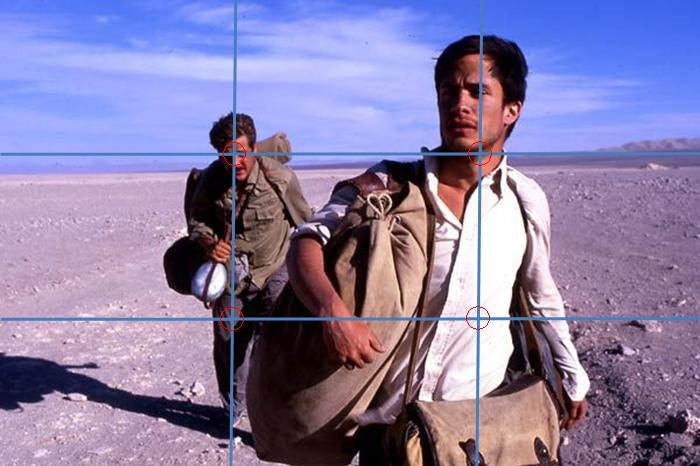
\includegraphics[scale=0.2]{img/image1.png}
\caption{Utilisation de la règle des tiers}
\label{fig:regle_tiers}
\end{figure}

Aussi, dans le cadrage, il n'y a pas que la règle tiers, les points forts et le balayage de l'image qu'il faut prendre. Il existe aussi un autre, c'est les lignes directrices. Ce sont des droite qui font "déplacer" l'oeil du spectateur. Les \textit{fuyantes} sont des lignes directrices qui vont accompagner l'oeil. Cela permet, entre autre, d'accentuer l'effet de perspective dans votre scène. Prenons la figure~\ref{fig:fuyante}, nous sommes sur une route de forêt. L'alignement des arbres et la route permettent de créer des fuyantes qui poussent l'oeil à regarder au loin et suivre la route. Dans certain cas, on peut aussi poser la fin d'un fuyante sur un point fort pour être sur que l'oeil se déplace vers ce point. 

\begin{figure}[h]
\centering
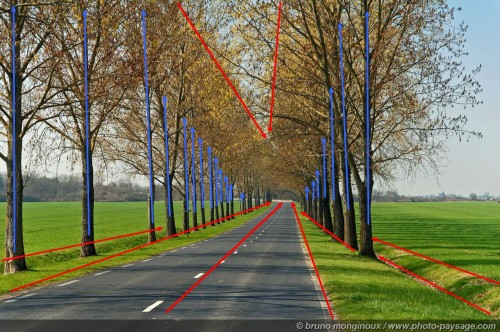
\includegraphics[scale=0.3]{img/image2.jpg}
\caption{Exemple de fuyantes}
\label{fig:fuyante}
\end{figure}

\smallskip

Une dernière chose, dans vos images essayer de bien equilibrer les masses, les volumes et les contrastes. Cela peut vite alourdir l'image et enlever toute la magie que vous vouliez faire passer.
\clearpage
	\subsection{Les valeurs de plan}
	\paragraph{Le plan d'ensemble}: le plan d'ensemble est un plan qui est beaucoup utiliser lorsque l'on a de beau paysages... Il sert principalement à situer les personnages et l'action. Il permet de préparer le spectateur à l'action qui va venir. Ce n'est le genre de plan que l'on va choisir lorseque l'on veut surprendre. 
	
\begin{figure}[h]
\centering
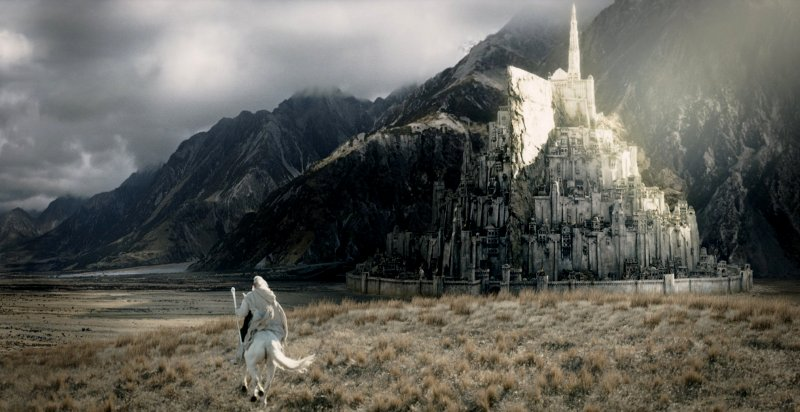
\includegraphics[scale=0.2]{img/plan1.png}
\caption{Le seigneur des anneaux}
\label{fig:regle_tiers}
\end{figure}

	\paragraph{Le plan général}: il est plus rapproché de l'action que le plan d'ensemble. Dans ce plan, on se concentre plus sur les personnages et sur l'action qui va arriver plutôt que sur le paysage et ce qui se passe en arrière plan. De nombreux réalisateurs choisissent de commencer leurs film par ce plan car il permet de mettre en place l'intrigue. Il aussi permettre de montrer une dernière fois le lieu où l'action. Je pense par exemple à une bataille entre chevaliers. A la fin de la bataille, le réalisateur peut choisir de faire un plan général pour montrer les concéquences de la bataille. 

\begin{figure}[h]
\centering
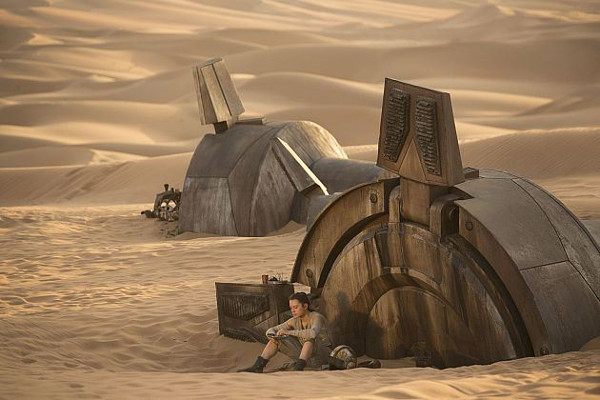
\includegraphics[scale=0.25]{img/plan2.jpg}
\caption{Star Wars}
\label{fig:regle_tiers}
\end{figure}

	\paragraph{Le plan en pied / moyen}: le plan moyen permet de posser l'action de façon plus significative que les plan larges (plan d'ensemble et plan général). Avec ce type de plan, on plus focaliser le spectateur sur les personnages et l'action qu'ils vont faire. On en donne plus d'informations extérieurs. La plupart du temps ce type de plan est utilisé dans des scènes d'actions.  
	
\begin{figure}[h]
\centering
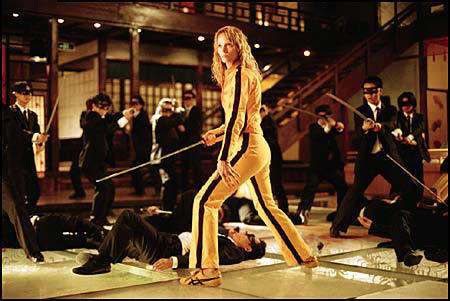
\includegraphics[scale=0.3]{img/plan3.png}
\caption{Kill Bill}
\label{fig:regle_tiers}
\end{figure}

\clearpage

	\paragraph{Le plan italien}: ce plan coupe le personnage au genou. Il est un plan caractéristique du cinéma italien d'où son nom. On pense que ce plan est dût à l'importance du genou en Italie. Ce plan est maintenant très peu utilisé, il a été remplacé par le plan americain.

\begin{figure}[h]
\centering
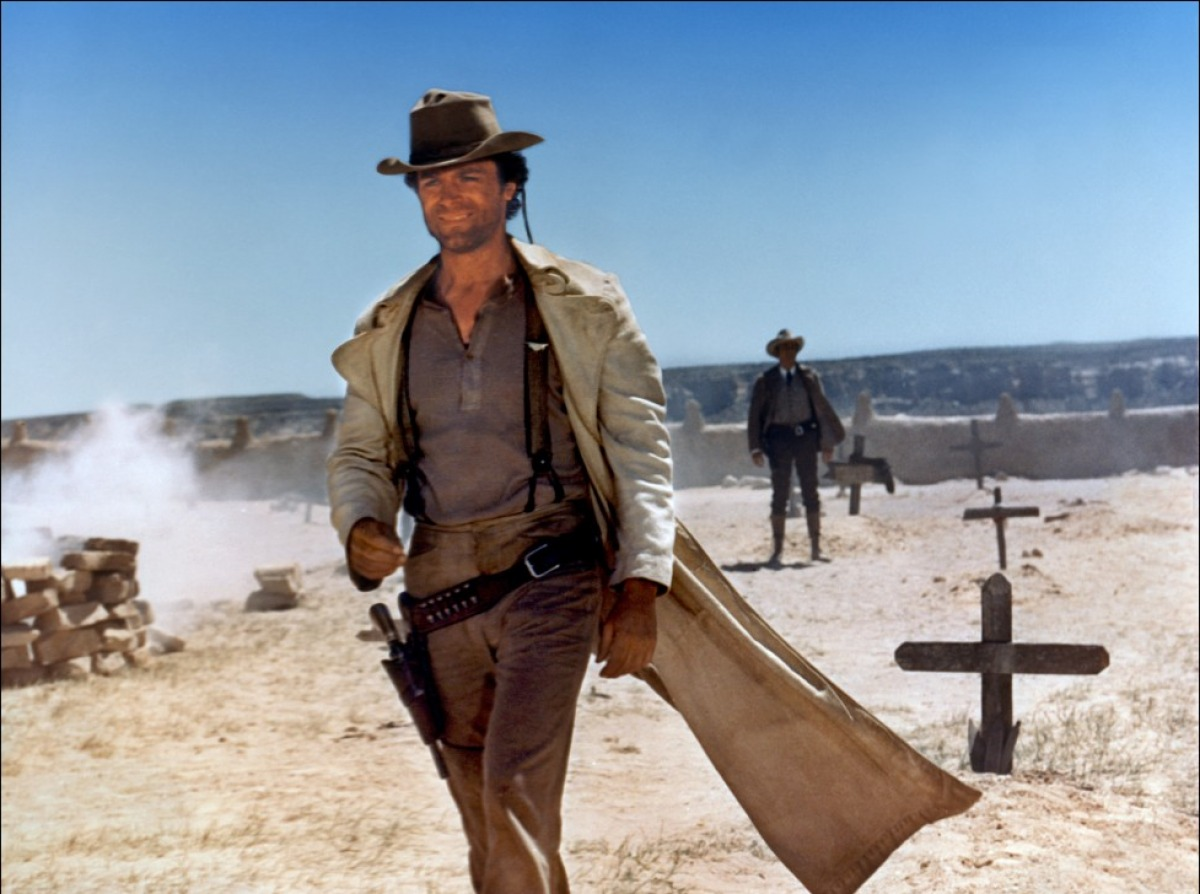
\includegraphics[scale=0.13]{img/plan4.jpg}
\caption{Pour une poignée de dollars}
\label{fig:regle_tiers}
\end{figure}

	\paragraph{Le plan américain}: ce plan vient de l'époque des western. Il fallait montrer les colts des cow-boys. Le cadreur devait mettre l'accent sur les revolvers, le plan est donc resté dans les annales du cinéma et maintenant c'est resté. Ce plan va rapprocher le spectateur du personnage, et son jeu d'acteur.

\begin{figure}[h]
\centering
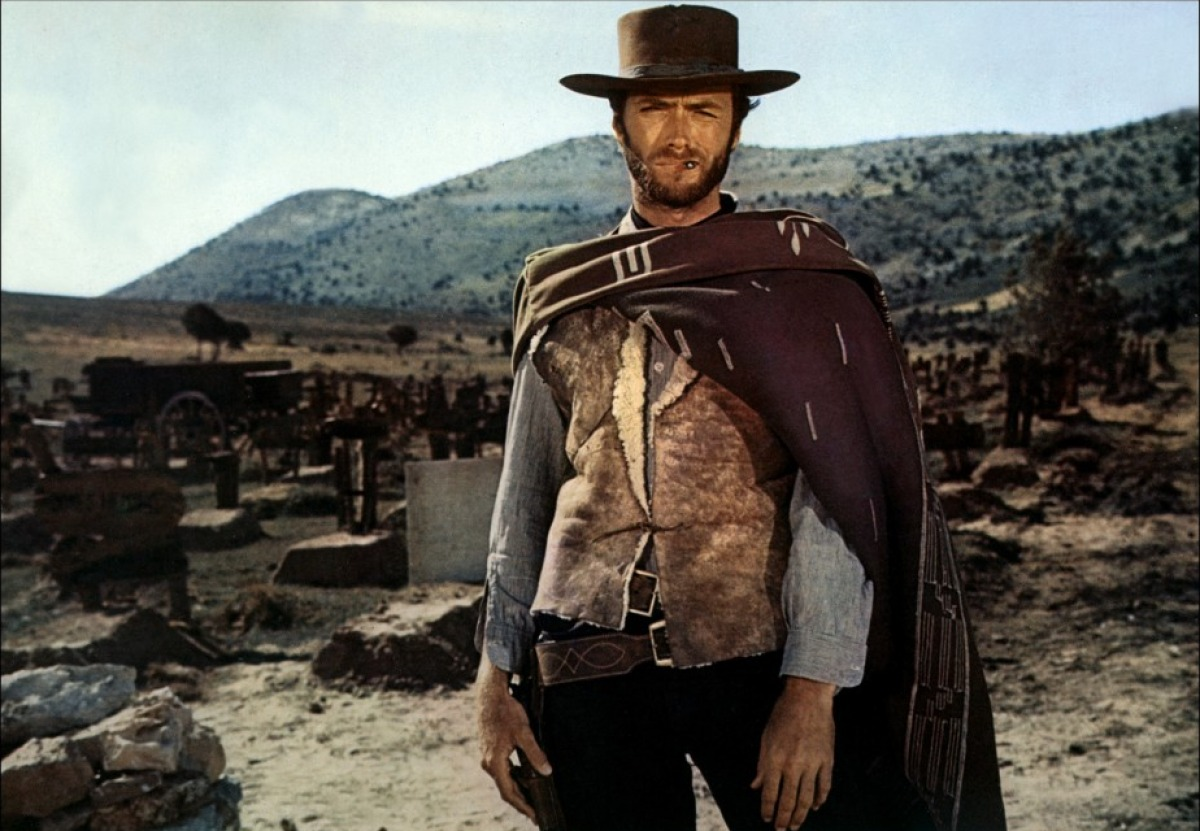
\includegraphics[scale=0.13]{img/plan5.jpg}
\caption{Pour une poignée de dollars}
\label{fig:regle_tiers}
\end{figure}

	\paragraph{Le plan taille} On coupe le cadrage au niveau de la taille. C'est un plan de séduction. Il peut aussi apporter la bagare. 

\begin{figure}[h]
\centering
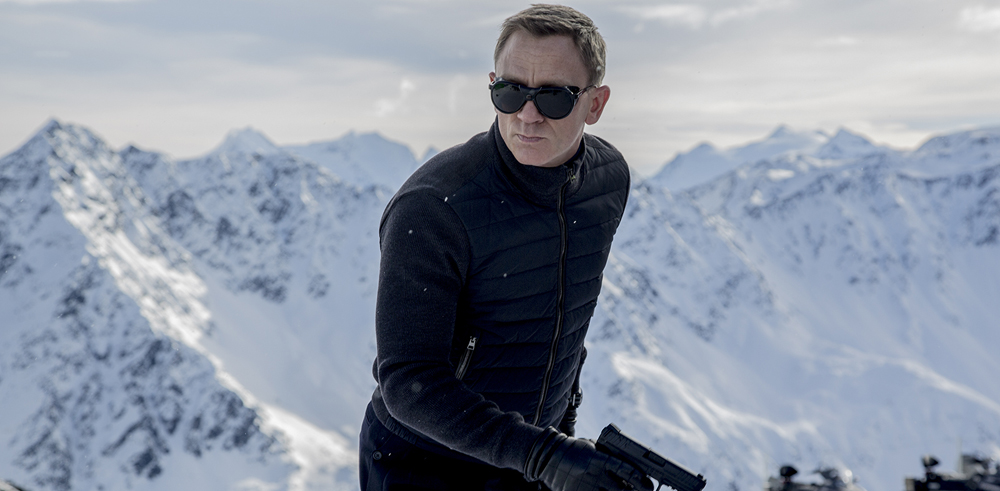
\includegraphics[scale=0.6]{img/plan6.jpg}
\caption{James Bond}
\label{fig:regle_tiers}
\end{figure}

\clearpage

	\paragraph{Le plan poitrine} Il est très utilisé en journalisme. C'est un plan intime.

\begin{figure}[h]
\centering
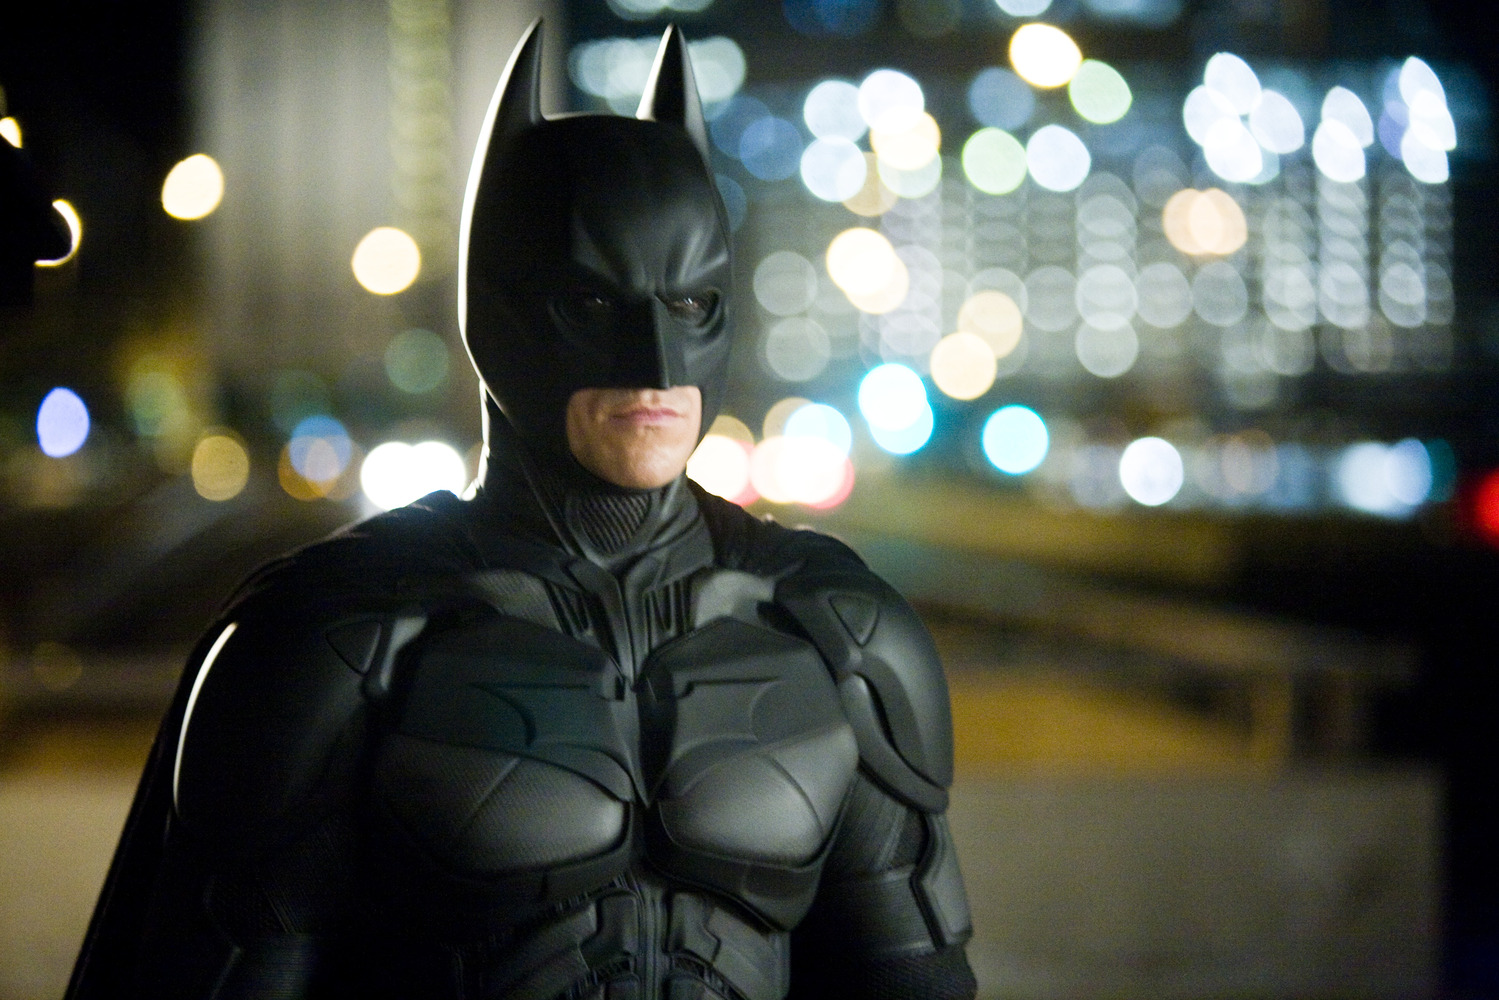
\includegraphics[scale=0.15]{img/plan7.png}
\caption{The Dark knight}
\label{fig:regle_tiers}
\end{figure}

	\paragraph{Le gros plan} Il permet de lire directement les émotions, ses réactions les plus intimes. C'est le plan de l'analyse psychologique, mais aussi celui de la sensualité ou de l'expressivité.

\begin{figure}[h]
\centering
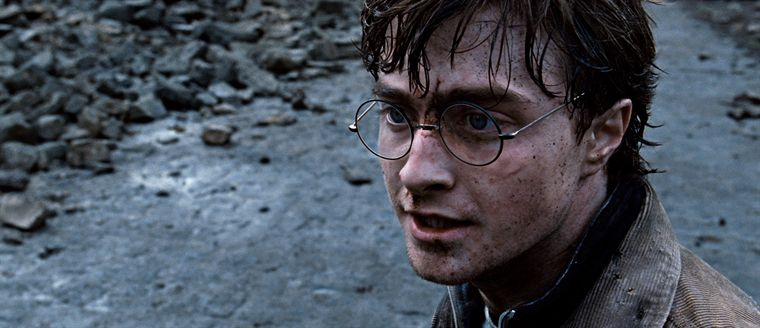
\includegraphics[scale=0.3]{img/plan8.jpg}
\caption{Harry Poter}
\label{fig:regle_tiers}
\end{figure}

	\paragraph{Le très gros plan} Il permet de montrer les yeux, la bouche, un élément du corps. Il permet de mettre l'accent sur un détail très important pour l'action passé ou à suivre.

\begin{figure}[h]
\centering
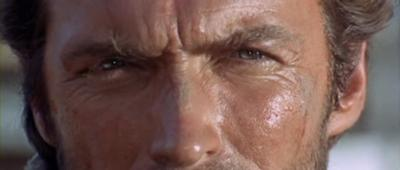
\includegraphics[scale=0.4]{img/plan9.jpg}
\caption{Pour une poignée de dollars}
\label{fig:regle_tiers}
\end{figure}

\smallskip

\clearpage
	
	\subsection{Les mouvements de caméra}
Comme pour les valeurs de plan, il existe plusieurs mouvements de caméras. Chacun a sa particularité, mais il faut savoir que le mouvement de caméra est avant tout un effet de technique, c'est lui qui permet la réalisation du plan. Il n'y a donc pas d'effets à travers les mouvements de caméras. Il faut plutôt réfléchir à quel plan le mouvement de caméra amène et donc après à quel effet le mouvement de caméra est associé.
\smallskip
Avant tout, il est bon de noter que les mouvements de caméras sont une invention récente du cinéma. En effet, à l'époque, les cadreurs devaient faire fonctionner la caméra en l'activant à l'aide d'une manivelle. Il était donc impossible de faire un mouvement de caméra. Les mouvements de caméras sont donc arrivés avec les premières caméras électriques. Il existe plusieurs mouvements de caméra.

	\paragraph{Les mouvements de caméra sans déplacement:}

\begin{enumerate}
	\item De gauche à droite
	\item De haut en bas
	\item En avant et en arrière
	\item Les rotations
\end{enumerate}

	\paragraph{Les mouvements de caméra avec déplacement:}
\begin{enumerate}
	\item La panoramique horizontale et verticale
	\item Le travelling latéral
	\item Le travelling horizontal
	\item Le travelling courbe
	\item Monter et descendre
\end{enumerate}

On peut aussi faire tourner la caméra sur son axe optique. Mais ce mouvement n'amène pas grand chose à l'histoire ou à la façon de la raconter. Un des grands film à ma connaissance qui s'est beaucoup servi de ce mouvement est Gravity. Dans ce film, on voulait absolument être dans l'espace et être immergé. Il fallait donc faire tourner la caméra.

\smallskip

\textit{Nota Bene : le zoom n'est pas un mouvement de caméra car il n'y a pas de changement de lignes de perspectives. C'est juste un aggrandissement de l'image.}

\clearpage

\section{Ecrire le film}
	\subsection{Le synopsis}

Le synopsis est un des textes qui est cense présenter à votre producteur l'idée principale que vous avez pour votre projet. Dans ce texte, il doit donc figurer tous les traits principaux de l'histoire, sans faire de descriptions précise des personnages. C'est un texte qui est censé à la fois vous faire réfléchir à synthétiser votre idée et aussi à la vendre. Un synopsis normal doit tenir dans une page, pas plus. Je vous ai laissé sur la page suivante un example de synopsis.

\clearpage

Luke Skywalker has vanished. In his absence, the sinister FIRST ORDER has risen from the ashes of the Empire and will not rest until Skywalker, the last Jedi, has been destroyed. With the support of the REPUBLIC, General Leia Organa leads a brave RESISTANCE. She is desperate to find her brother Luke and gain his help in restoring peace and justice to the galaxy. Leia has sent her most daring pilot on a secret mission to Jakku, where an old ally has discovered a clue to Lukes whereabouts.

The First Order, led by the evil Kylo Ren, is landing stormtroopers to attack a small village, as Poe Dameron meets with Lor San Tekka in a hut. He is given a small bag containing the map to Luke Skywalker. Kylo Ren orders the stormtroopers to destroy Lor San Tekka's entire village and takes Poe captive. Captain Phasma, a stormtrooper wearing chrome-plated armor, leads the attack. Kylo Ren wears a black mask and uses a red, fiery lightsaber. Poe's X-Wing is damaged so that he cannot escape, so the pilot puts the map in a rolling droid unit called BB-8. He fires at Kylo Ren, who uses the Force to block a blaster bolt. As Dameron is captured, the troopers massacre the prisoners, but one stormtrooper FN-2187, refuses to fire. Meanwhile BB-8 rolls away across the sands, narrowly escaping capture. The droid runs into Rey, a young scavenger who is barely surviving on Jakku. Rey scavenges parts from old wrecks of Star Destroyers on the sands of Jakku, and exchanges them for food at Unkar Plutt's scrap yard. The marks on the walls of her hut indicate she's been on Jakku for a very long time. She rescues BB-8 from a Teedo scavenger. She can understand his beeps and whistles, and offers him shelter for the night.

On the First Order destroyer, Poe is unsuccessfully interrogated by the First Order. Kylo Ren is called in to use his Force powers to extract information from Poe about the whereabouts of the map. Poe resists, but ultimately divulges that the map is still on Jakku in his BB-8 unit.

Meanwhile Captain Phasma confronts FN-2187 about his behavior on Jakku. She orders him to take his unused blaster in for inspection and report to her division and ultimately reconditioning. Instead FN-2187 decides to run away. He needs a pilot to escape the star destroyer, so he rescues Poe, and the two board a black First Order TIE fighter and escape. Poe renames FN-2187 as Finn, and expertly pilots to an escape while Finn fires the ship's blasters. The fighter is hit by lasers from the destroyer and crash lands on Jakku. Finn has ejected but it appears Poe has gone down with the ship leaving only his jacket.

Finn wanders across the desert discarding his stormtrooper armor. Eventually, he arrives in Niima Outpost, the town where Rey trades scrap for food. While Finn is looking for water in the town, he sees Rey being accosted by two of Unkar Plutt's henchmen who are trying to make off with BB-8. He begins to rush to her aid, but before he gets far, Rey handily fights off her attackers using her staff. Clearly, she can handle herself. BB-8 spots Finn looking their way, and tells Rey that he is wearing Poe's jacket which they assume is stolen. Rey chases Finn down, knocks him to the ground and confronts Finn about the jacket. Finn tells them that Poe was captured by the First Order and that he helped him escape, but Poe was unfortunately killed. BB-8 is saddened and rolls off , but Rey is excited and impressed, and assumes Finn is a resistance fighter. Finn lies, telling her he is indeed with the resistance. Rey excitedly tells Finn that BB-8 is on a secret mission. Finn tells her BB-8 is carrying a map to Luke Skywalker and Rey is even more impressed, declaring that she thought Skywalker was a myth.

BB-8 returns and alerts Finn and Rey that they are in trouble. First Order stormtroopers are now looking for Finn and the BB-8 droid. Stormtroopers chase Finn, Rey and BB-8 through Niima Outpost and TIE fighters are called in and begin to bomb and strafe the town. To make their escape, they steal a "garbage" vehicle to escape the First Order. It is the Millennium Falcon. Rey takes the pilot's seat while Finn mans the guns. Neither is confident in their abilities, and their lift off is rough, destroying a substantial portion of the town as they try to get off of the ground. Finn is able to shoot down a pursuing fighter, but the guns are hit and locked in a position that prevents him from taking out the remaining fighter. Rey flies through the wrecked ships in the desert of Jakku, occasionally scraping through the sands as they try to keep low to confuse the TIE fighter's tracking. Rey takes the Falcon into one of the Star Destroyers and just as the pursuing fighter locks onto their ship, she turns the Falcon out into the open, and performs a flip which allows Finn to fire successfully at the remaining fighter, taking it down. They head off, away from Jakku, and on toward the wider galaxy. Not having flown in years, the Falcon is not in good repair, and almost immediately requires an emergency patch. Rey begins repairing the ship while Finn admits to BB-8 he is not part of the resistance, but is still able to convince BB-8 to tell them where the Resistance base is.
\medskip

\textit{Je ne vous ai mis que le tier du synopsis. C'est juste pour vous donner une idée de la longueur d'un sysnposis fâce à celle d'un scènario (voir celui d'Interstellar)}

\clearpage

	\subsection{Le scènario}
Le scénario est l'étape la plus importante d'un film. Le film a (a priori été vendu au producteur) été vendu. Le but d'un scénario est de faire passer dans tous les détails, l'histoire, la visée et le but du film. Si un scénario est mal écrit, les équipes de story-board ne pourront pas vraiment bien comprendre ce qu'il faut dessiner... et cela a un effet domino. Tout peu s'écrouler par un scénario mal écrit. Dans un scénario, il y a plein de consignes et régles à respecter. Par commencer la présentation. C'est un peu l'une des seule régles, mais elle est très importante. 

\medskip

Tout d'abord, les scènes (l'endroit où se passe l'action) sont écrites d'une manière spéciale. On écrira INT ou EXT en fonction de la localisation de la scène (INT pour une scène en INTérieur et EXT pour une scène en EXTérieur). Ensuite, on ajoute le lieu de l'action. Il faut indiquer les lieux de façon présise (si besoin est).
Ensuite, il faut écrire ce que voit et entend la caméra. On notera \textit{que} ce que voit et entend la caméra. C'est à dire rien de l'ordre psycologique.
 Enfin, on écrit le dialogue. On écrit le nom de l'acteur au centre de la feuille et s'en suit le discours. On ajoute OFF si le personnage est en voix off. Si une personnage entre en scène, il faut l'introduire. Lorseque la scène comporte plus de 2 personnages, on devra écrire à qui le personnage s'adresse. On notera aussi la transition, les plus courantes sont le CUT et le FADE OUT. 

Pour que vous compreniez mieux comment on structure un scènario, je vous invite à vous rendre sur le site de l'IMSDb qui vous propose les scénario de la plupart des films connus. Cela vous permettra de vous mettre en tête la façon d'écrire un scénario.


\begin{figure}[h]
\centering
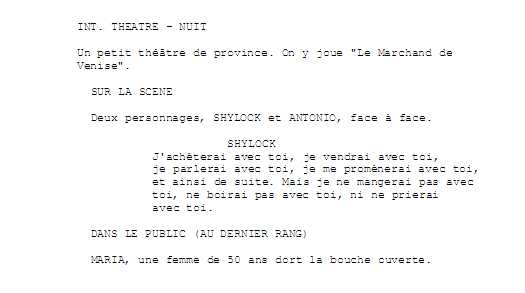
\includegraphics[scale=0.7]{img/scenario.jpg}
\caption{Exemple de scénario lambda}
\label{fig:scena}
\end{figure}

\clearpage


	\subsection{le story-board}
\label{sec:story}

le story board est d'après moi le moment le plus amusant de l'écriture d'un film. C'est le moment où vous allez mettre en place tout ce qui est VFX et objets hors du commun. Vous allez en réalité, dessiner ce que doit voir la caméra. Cela permet de mettre sur papier "l'âme" du film. C'est une étape importante aussi, il n'y a pas vraiment de régles. Le but du story-board est d'être compris par tous, il faut donc le faire le plus compréhensif possible. Le but n'est pas ici de faire de beau dessins mais de montrer au cadreur et à toutes les équipes de post-production ce que le scénariste n'aurait pas pu écrire. Il n'y a pas de dialogue dans un story-board.

Je vous ai mis un de mes story-board préféré. Celui de Star-wars. :D

\begin{figure}[p]
\centering
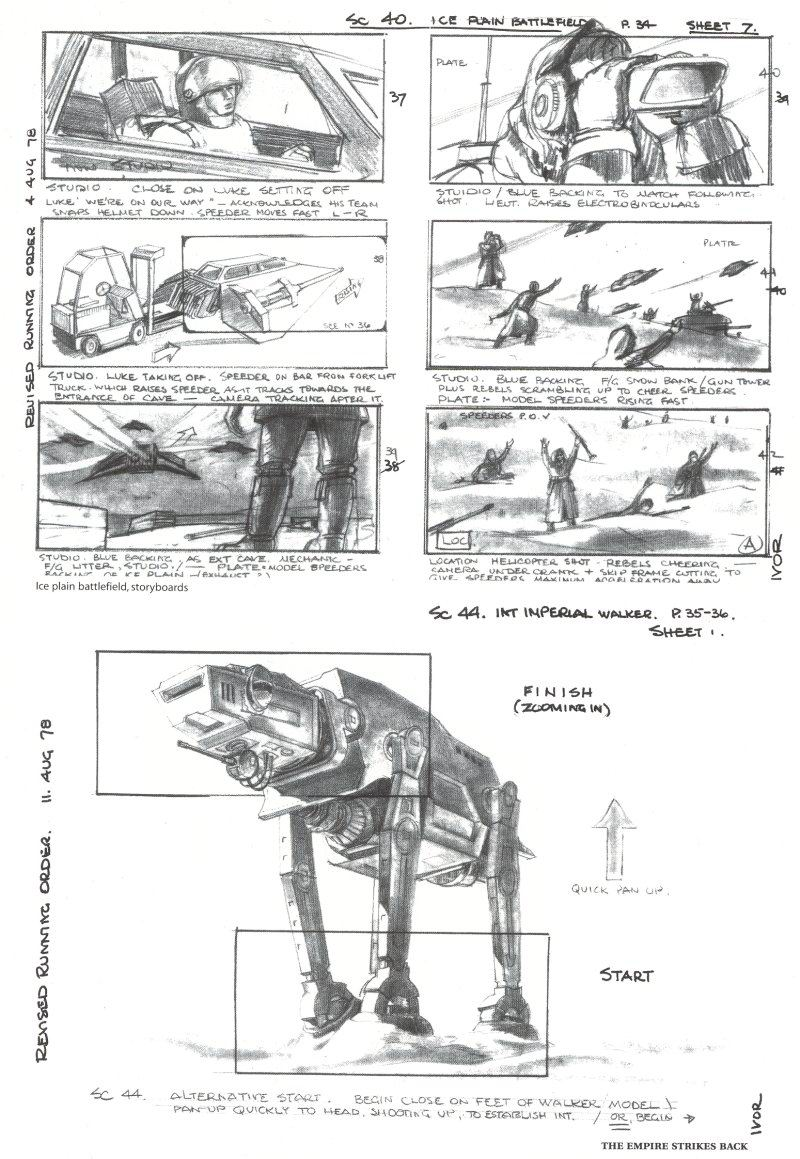
\includegraphics[scale=0.5]{img/story.jpg}
\caption{Exemple de story board}
\label{fig:story}
\end{figure}

\clearpage

	\subsection{Le diagramme de Gantt}

Le diagramme de Gantt n'est pas indispensable à la production d'un film. Il permet juste d'organiser le plateau au maximum. Il permet de gérer les imprévus, de gérer le temps... Je vous ai mis un exemple de diagramme de Gantt dessous. Si vous voulez absoluement faire un diagramme de Gantt, je vous invite à utiliser le logiciel GanttProject. 

\begin{figure}[h]
\centering
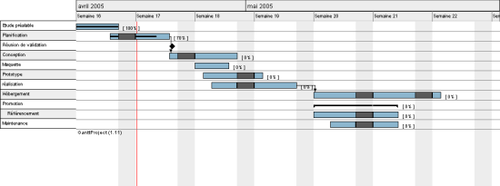
\includegraphics[scale=0.5]{img/gantt.png}
\caption{Exemple de diagramme de Gantt}
\label{fig:story}
\end{figure}

\bigbreak

\bigbreak
\bigbreak
\bigbreak
\bigbreak
\bigbreak

\bigbreak
\bigbreak
\bigbreak
\bigbreak
\bigbreak
\bigbreak
\bigbreak
\bigbreak
\bigbreak
\bigbreak

\textit{écrit par Paul Planchon - 2016. Source disponible à la demande. :)}


\end{document}

